\documentclass[12pt]{article}
% \documentclass{article}
\usepackage{amsmath}
\usepackage{graphicx} 
% \usepackage{graphicx,subfigure}
\usepackage{caption}
\usepackage[scheme=plain]{ctex}
\pagestyle{empty}
\usepackage{amsmath,times,bm,hyperref}
\usepackage{amssymb}
\usepackage{listings}
\usepackage{xcolor}
\lstset { %
    language=C++,
    backgroundcolor=\color{black!5}, % set backgroundcolor
    basicstyle=\footnotesize,% basic font setting
}
\hypersetup{
colorlinks=true,
linkcolor=black
}


%%%%%%%%%%%%%%%%%%%%%%%%%%%%%%%%%%%%%%%%%%%%%%%%%%
% Do not modify the dimensions of the page
\setlength{\topmargin}{0mm}
\setlength{\headheight}{0mm}
\setlength{\headsep}{0mm}
%% 25.4 -25.4 = 0
\setlength{\topmargin}{0mm}
%% 25.4 -25.4 = 0
\setlength{\oddsidemargin}{0mm}
%% 210 -25(left) -25(right) = 160
\setlength{\textwidth}{160mm}
%% 297 -25(top) -30(bottom) = 242
\setlength{\textheight}{242mm}
\setlength{\parindent}{0pt}
\setlength{\parskip}{12pt}
% Do not modify the dimensions of the page
%%%%%%%%%%%%%%%%%%%%%%%%%%%%%%%%%%%%%%%%%%%%%%%%%%

\begin{document}

\title{\bf MAE5032 Final Project}
\author{Qiang Li}
\date{\today}
\maketitle

\section*{1. Problem}
We consider the transient heat equation in a one-dimensional (1D) domain $\Omega := (0,1)$. The boundary of the domain is $\Gamma = \left\lbrace 0, 1 \right\rbrace$.
Let $f$ be the heat supply per unit volume, $u$ be the temperature,  $\rho$ be the density, $c$ be the heat capacity, $u_0$ be the initial temperature, $\kappa$ be the conductivity, $n_x$ be the Cartesian components of the unit outward normal vector . The boundary data involves the prescribed temperature $g$ on $\Gamma_g$ and heat flux $h$ on $\Gamma_h$. The boundary $\Gamma$ admits a non-overlapping decomposition: $\Gamma = \overline{\Gamma_{g} \cup \Gamma_h}$ and $\emptyset = \Gamma_g \cap \Gamma_h$. The transient heat equation may be stated as follows.

\begin{align*}
\rho c \frac{\partial u}{\partial t} - \kappa  \frac{\partial^2 u}{\partial x^2} &= f \quad \mbox{ on } \Omega \times (0,T) \\
u &= g \quad \mbox{ on } \Gamma_{g} \times (0,T) \\
\kappa \frac{\partial u}{\partial x} n_{x}  &= h \quad \mbox{ on } \Gamma_h \times (0,T) \\
u|_{t=0} &= u_0 \quad \mbox{ in } \Omega.
\end{align*}

\section*{2. Theoretical analysis}
\subsection*{2.1 Explicit Euler method}
\begin{equation}
    \frac{\partial u}{\partial t}=\frac{u^{n+1}-u^n}{\Delta t}+O(\Delta t^2)\label{partial time}
\end{equation}
\begin{equation}
    \frac{\partial^2 u}{\partial x^2}=\frac{u_{i+1}-2u_i+u_{i-1}}{\Delta x^2}+O(\Delta x^3)\label{partial u}
\end{equation}
With FDM, the transient heat equation in 1D can be dispersed into the following:
\begin{equation}
    u^{n+1}=u^n+\frac{\kappa\Delta t}{\rho c\Delta x^2}(u_{i+1}^n-2u_i^n+u_{i-1}^n)+\frac{f\Delta t}{\rho c}\label{3}
\end{equation}

So we can get a tri-diagonal system $AX+X1=b$:
\begin{center}
\begin{pmatrix}
b & a & 0 & ... & 0 \\
a & b & a \\
 & & ... & \\
 &  & a & b & a\\
0 & 0 & ... & a & b
\end{pmatrix}\begin{pmatrix}
u_1^{n} \\
u_2^{1} \\
. \\
. \\
u_m^{n}
\end{pmatrix}+$\frac{f\Delta t}{\rho c}$=\begin{pmatrix}
u_1^{n+1} \\
u_2^{n+1} \\
. \\
. \\
u_m^{n+1}
\end{pmatrix}
\end{center}
\begin{equation*}
    a=\frac{\kappa\Delta t}{\rho c\Delta x^2}, b=1-2\frac{\kappa\Delta t}{\rho c\Delta x^2}
\end{equation*}


\subsection*{2.2 Implicit Euler method}
From eq. \ref{partial time} and eq. \ref{partial u}, we can deduce the following:
\begin{equation}
    \rho c\frac{u_i^{n+1}-u_i^n}{\Delta t}-\kappa\frac{u_{i+1}^{n+1}-2u_i^{n+1}+u_{i-1}^{n+1}}{\Delta x^2}=f
\end{equation}
\begin{equation}
    -\frac{\kappa\Delta t}{\rho c\Delta x^2}u_{i+1}^{n+1}+(1+2\frac{\kappa\Delta t}{\rho c\Delta x^2})u_i^{n+1}-\frac{\kappa\Delta t}{\rho c\Delta x^2}u_{i-1}^{n+1}=u_i^n+\frac{f\Delta t}{\rho c}\label{5}
\end{equation}

So we can get a tri-diagonal system $AX=b$:
\begin{center}
\begin{pmatrix}
b & a & 0 & ... & 0 \\
a & b & a \\
 & & ... & \\
 &  & a & b & a\\
0 & 0 & ... & a & b
\end{pmatrix}\begin{pmatrix}
u_1^{n+1} \\
u_2^{n+1} \\
. \\
. \\
u_m^{n+1}
\end{pmatrix}=\begin{pmatrix}
u_1^n+\frac{f\Delta t}{\rho c} \\
u_2^n+\frac{f\Delta t}{\rho c} \\
. \\
. \\
u_m^{n}+\frac{f\Delta t}{\rho c}
\end{pmatrix}\\
 \end{center}
\begin{equation*}
    a=-\frac{\kappa\Delta t}{\rho c\Delta x^2}, b=1+2\frac{\kappa\Delta t}{\rho c\Delta x^2}
\end{equation*}

\subsection*{2.3 Exact solution}
Because $\frac{\partial u}{\partial t}=0$ , so we can get exact solution by integration.
\begin{equation}
    u_{exact} = \frac{sin\pi x}{\pi^2}
\end{equation}

\subsection*{2.4 Stability analysis(Von Neumann)}
\subsubsection*{2.4.1 Explicit scheme}
Let $\kappa=\rho=c=1.0,cfl=\frac{\Delta t}{\Delta x^2}$, so the Eq. \ref{3} can rewrite:
\begin{equation}
    u^{n+1}=u^n+cfl(u_{i+1}^n-2u_i^n+u_{i-1}^n)\label{7}
\end{equation}
With Von Neumann,we can get by Eq. \ref{7}:
\begin{equation}
    e^{\sigma\Delta t}=1-2cfl + cfl(e^{ik\Delta x}+e^{-ik\Delta x})\label{8}
\end{equation}
Simply Eq. \ref{8}:
\begin{equation}
     e^{\sigma\Delta t}=1-2cfl+2cflcos(k\Delta x)
\end{equation}
\begin{equation*}
    |e^{\sigma\Delta t}|\leq 1\to 0\leq cfl \leq \frac{1}{2}
\end{equation*}
So the explicit scheme is conditional stable, the conditional is that $0 \leq cfl \leq \frac{1}{2}$.

\subsubsection*{2.4.2 Implicit scheme}
Similarly with 2.4.1, Eq. \ref{5} can rewrite:
\begin{equation}
    -cflu_{i+1}^{n+1}+(1+2cfl)u_i^{n+1}-cflu_{i-1}^{n+1}=u_i^n\label{10}
\end{equation}
With Von Neumann,we can get by Eq. \ref{10}:
\begin{equation}
    -cfle^{\sigma\Delta tik\Delta x}+(1+2cfl)e^{\sigma\Delta t}-cfle^{\sigma\Delta t-ik\Delta x}=1\label{11}
\end{equation}
Simply Eq. \ref{11}:
\begin{equation*}
    e^{\sigma\Delta t}=\frac{1}{1+2cfl-2cflcos(k\Delta x)}\leq 1
\end{equation*}
So the implicit scheme is unconditional stable.

\section*{3. Code analysis}
\begin{figure}
    \centering
    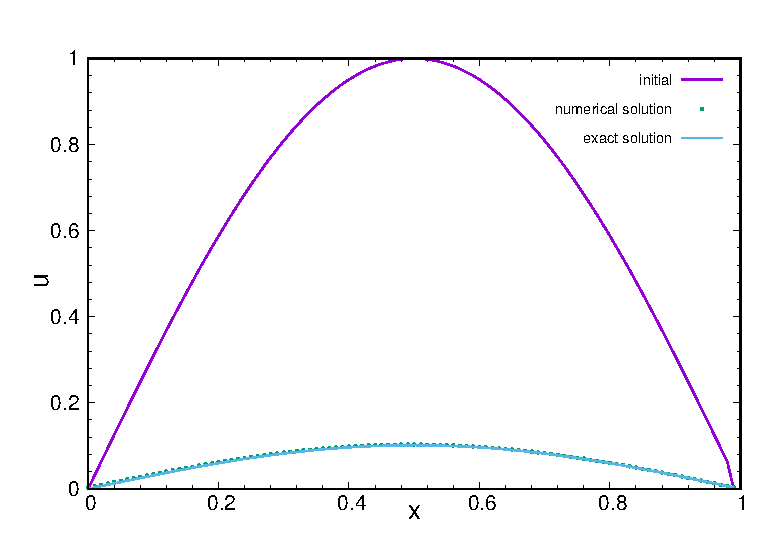
\includegraphics{img/explicit.eps}
    \caption{explicit scheme result with initial }
    \label{fig:explicit}
\end{figure}

\begin{figure}
    \centering
    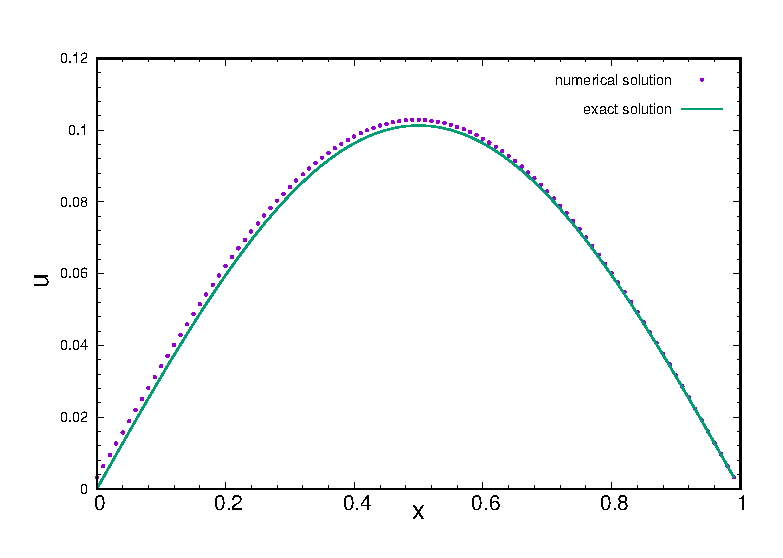
\includegraphics{img/explicit1.eps}
    \caption{explicit scheme result}
    \label{fig:explicit1}
\end{figure}

\begin{figure}
    \centering
    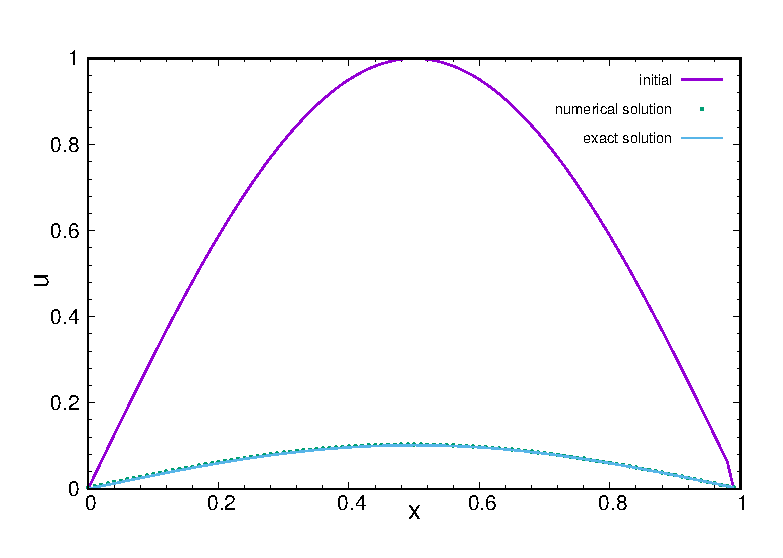
\includegraphics{img/implicit.eps}
    \caption{implicit scheme result with initial}
    \label{fig:implicit}
\end{figure}

\begin{figure}
    \centering
    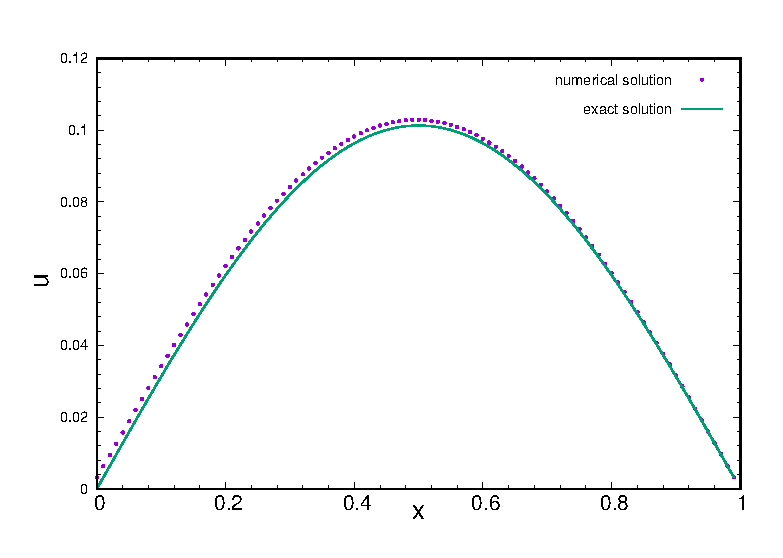
\includegraphics{img/implicit1.eps}
    \caption{implicit scheme result }
    \label{fig:implicit1}
\end{figure}

\begin{figure}
    \centering
    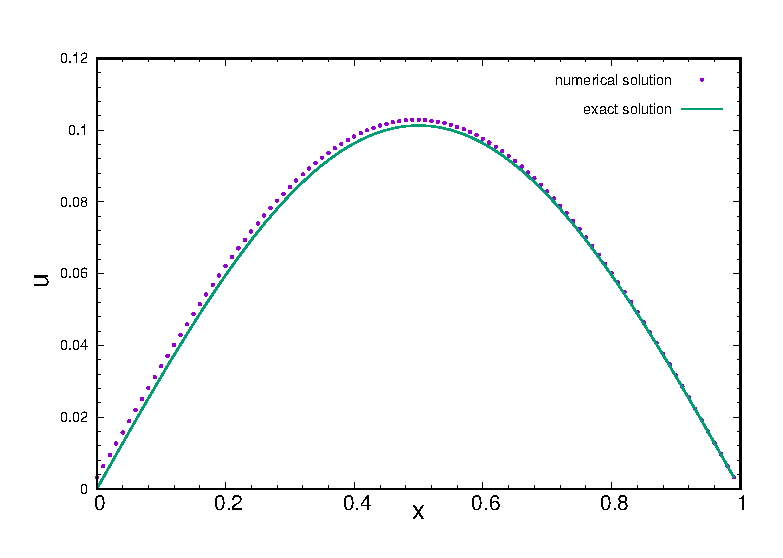
\includegraphics{img/t00005.eps}
    \caption{dt=0.00005}
    \label{fig:t00005}
\end{figure}

\subsection*{3.1 Code result}
When $\Delta t=0.00002,\Delta x= 0.01$,Fig \ref{fig:explicit} to Fig \ref{fig:implicit} are the results after calculating 100000 steps (t=2s). And the two results are nearly same with the exact solution. So we can deduce we get the exciting results.\\
When $\Delta t=0.00006,\Delta x= 0.01$, the result can not deliver stable calculations in explicit scheme. So i choose $\Delta t=0.00005$ as the maximum time step in explicit scheme. As show in Fig. \ref{fig:t00005},the result is nearly match with the theoretical analysis. Because implicit scheme is unconditional stable, so it always can deliver stable calculations.

\subsection*{3.2 Profiling analysis}
\begin{figure}
    \centering
    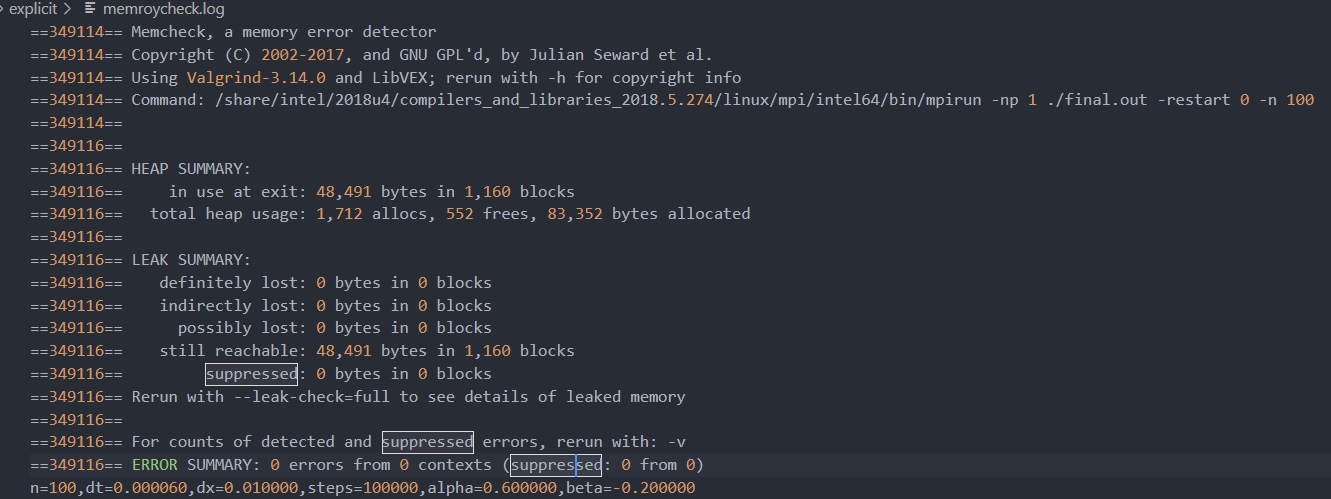
\includegraphics[scale=0.5]{img/profileexp.png}
    \caption{The profile analysis with valgrind for explicit scheme}
    \label{fig:profileexp}
\end{figure}

\begin{figure}
    \centering
    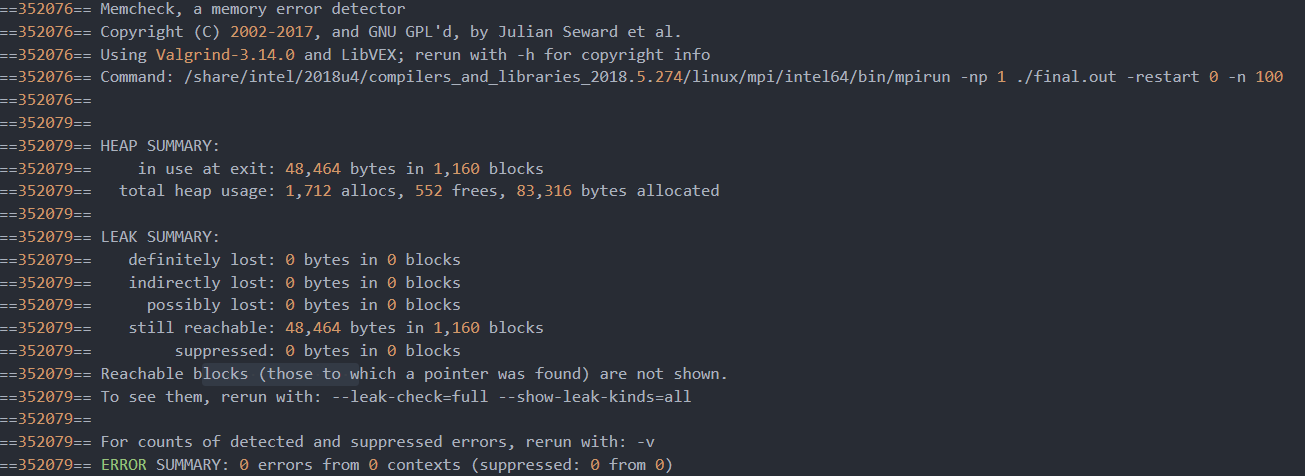
\includegraphics[scale=0.5]{img/profileimp.png}
    \caption{The profile analysis with valgrind for implicit scheme}
    \label{fig:profileimp}
\end{figure}

Fig. \ref{fig:profileexp} and Fig. \ref{fig:profileimp} are the profile analysis with valrgirnd for explicit and implicit program.As the two figures show, although we destroyed all petsc variables , etc mat,vec and ksp and so on , there are many heap didn't be freed.I guess those are built in malloc memory in petsc.


\subsection*{3.3 Parallel analysis}
Fig. \ref{fig:time} is the time cost with the number of processors increases. But the result is contrary to our expectation. We expect that the time should be reduced as the number of processors increases. And the Fig. \ref{fig:flops} also show the unfortunate result that with the number of processors increases,the computing power is declining.I guess that with the number of processor increase, significant increase in communication time between processors. Therefore, it can be considered that the parallel effect of this program is not ideal.

\begin{figure}
    \centering
    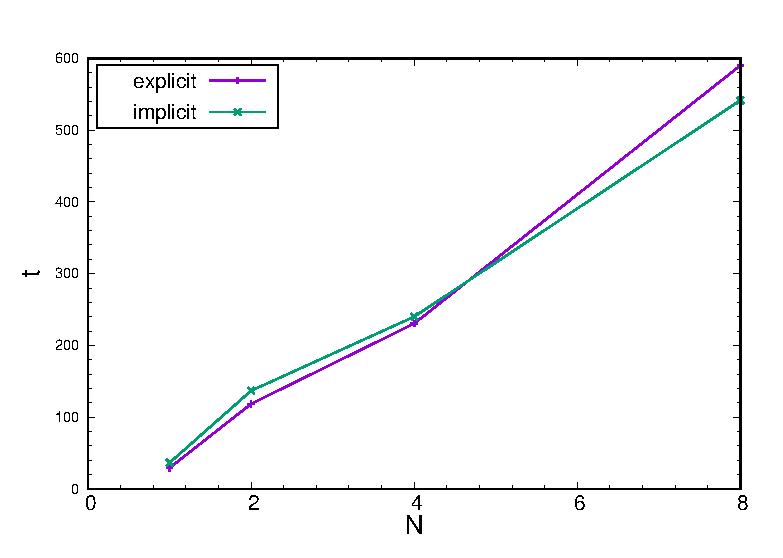
\includegraphics{img/time.eps}
    \caption{Time cost}
    \label{fig:time}
\end{figure}

\begin{figure}
    \centering
    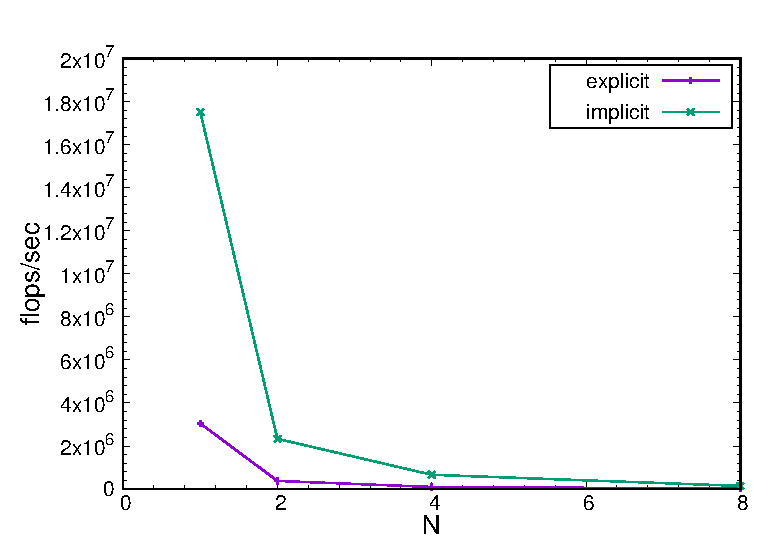
\includegraphics{img/flops.eps}
    \caption{Flops/sec}
    \label{fig:flops}
\end{figure}


\subsection*{3.4 Comparison between different ksp and pc}


\begin{figure}
    \centering
    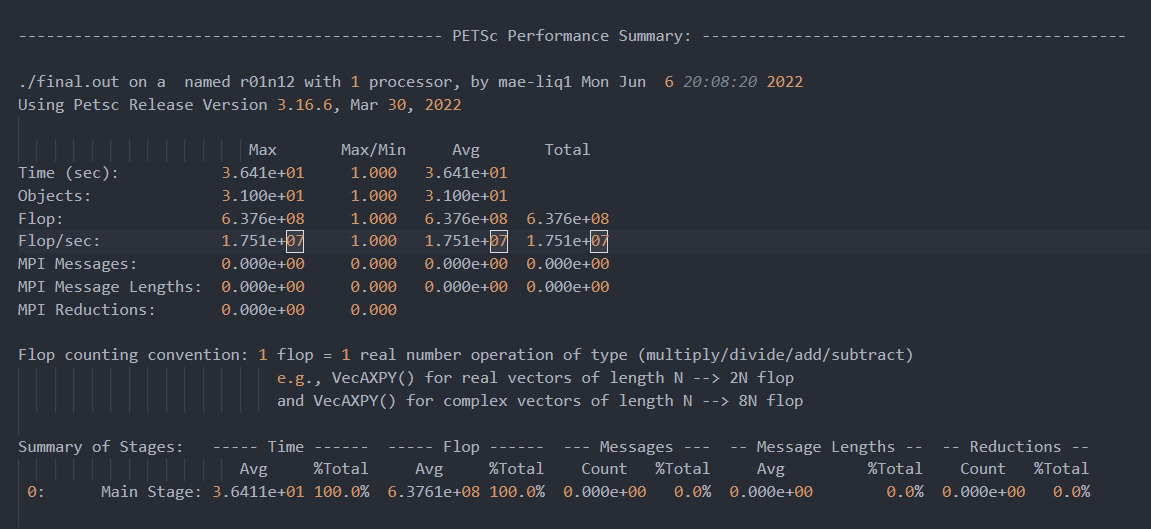
\includegraphics[scale=0.6]{img/ksp-default1.png}
    \caption{the performance Summary for ksp=DEFAULT,pc=PCJACOBI}
    \label{fig:ksp-default1}
\end{figure}

\begin{figure}
    \centering
    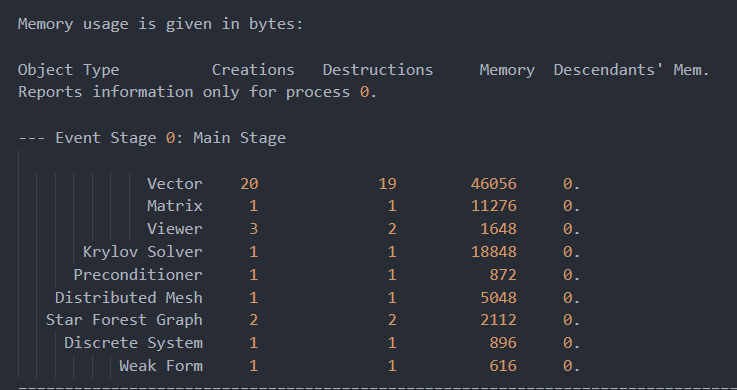
\includegraphics[scale=0.8]{img/ks-default2.png}
    \caption{the memory usage for ksp=DEFAULT,pc=PCJACOBI}
    \label{fig:ksp-default2}
\end{figure}

\begin{figure}
    \centering
    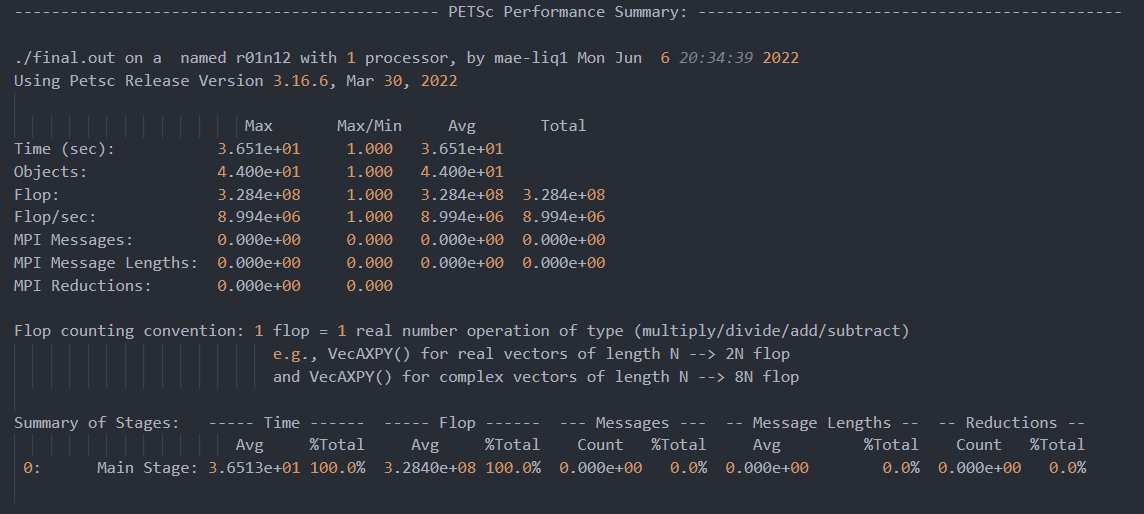
\includegraphics[scale=0.6]{img/ksp-germ1.png}
    \caption{the performance summary for ksp=gmres,pc=asm}
    \label{fig:ksp-gmres1}
\end{figure}

\begin{figure}
    \centering
    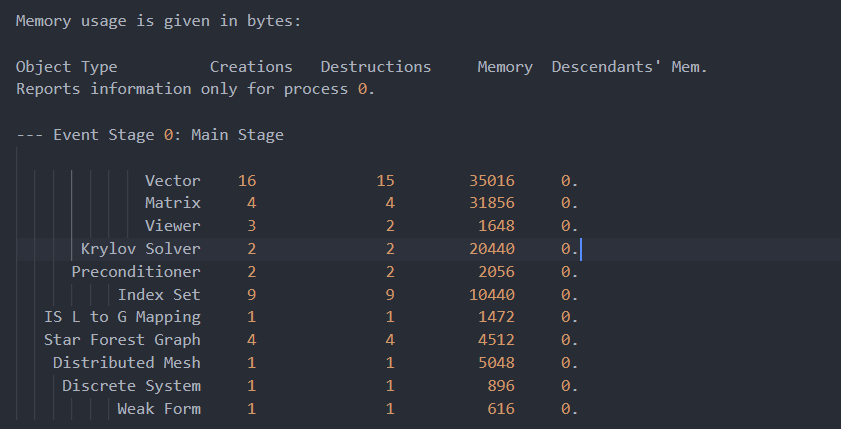
\includegraphics[scale=0.8]{img/ksp-germs2.png}
    \caption{the memory usage for ksp=gmres,pc=asm}
    \label{fig:ksp-gmres2}
\end{figure}


Because this program don't have a good parallel capability,so I chose one processors to compare different ksp and pc. Fig. \ref{fig:ksp-default1} and Fig. \ref{fig:ksp-default2} is profile analysis for ksp=Default,pc=pcjacobi, and Fig. \ref{fig:ksp-gmres1} and \ref{fig:ksp-gmres2} is profile analysis for ksp=gmres,pc=asm.As these figure show, performance of  jacobi is greater than asm(etc time,flop/sec and memory usage).



\section*{4. Conclusion}
We can get a numerical solution which is nearly same with exact solution.Explicit scheme is conditional stable and implicit scheme is unconditional stable.The program realized many tasks for this program but the parallelism ,which isn't good.\\
Finally,through this project,I have a deeper understanding of finite difference methods, Makefile, gnuplot, latex, and PETSc.

\end{document}